\chapter{Realisation}

\section{Light Display Shape}
\label{LEDshape}
As a first step possible shapes and places for the illumination were sketched on paper and then prototyped in full size with cardboard. The light should be visible in peripheral vision via reflections in the car interior. Thus the placement should be so that the light reaches the whole cabin, but does not obstruct the view. A cardboard ellipse with the width and height shown in Equation 3.1 filled average sized car cabins quite well. 
\begin{equation}2\pi \sqrt[]{\frac{\frac{113 cm}{2}^2 * \frac{140 cm}{2}^2}{2}}\approx 400cm \end{equation}
An ellipse is the ideal shape as it surrounds the passengers 360° and uses the maximal ceiling space without corners or bends.

\section{The human eye}
\label{sec:eye}
Some properties of the human eye and visual system need to be considered for the design of the ambient display. In \cite{Wordenweber2007AutomotiveVision} properties of the human eye that are relevant to the design of vehicle lighting (exterior and interior lighting) are presented. 
Lightness refers to perceived intensity of a color in relation to its illuminated context, whereas brightness refers to a sensation of absolute achromatic intensity\cite{Brill2014DoesQuestion}. Human eyes can operate over a large range of brightness because humans do not perceive light linearly but logarithmic (Weber–Fechner law\footnote{\url{https://learn.sparkfun.com/tutorials/light/visible-light}}.

Cone cells, which are more densely distributed in the center of the eye, are more sensitive to colors, whereas rod cells, which are found concentrated at the outer edges of the retina, are more sensitive in general but not to color.

\section{LED considerations}
\label{LEDconsiderations}
The automotive industry is very concerned about revenue per item. Especially suppliers must take care that they are competitive. LED strips are widely available from chinese suppliers for very competitive prices. The most popular addressable LEDs are those with the integrated WS2812B microcontroller. Each of the pixels has one red, green and blue led that can all be controlled from a single data cable. The american do-it-yourself manufacturer Adafruit sells them as Neopixel, and provides good documentation about their possibilities and restrictions. LEDs with the microprocessor SK6812 often have an additional white LED. This fourth colour is necessary for natural white light as red, green and blue from LEDs usually do not mix a pleasant white. Adafruit sells these LEDs as Neopixels too; this is a bit misleading because they use a slightly different protocol as the they have another 8-bit channel in the data signal for the white component of each pixel. As the light bar is planned not just to deliver light signals but also work as a reading light and room lightning a white component is necessary. There is also addressable LEDs with the APA102 available, they run a lot faster (20Khz vs 600 Hz) but are also less economically. Adafruit brands them as DotStar. 

The LEDstrips are widely available with densities of 30, 60 and 144 Pixels per meter.
With the amount of pixels there are a few tradeoff to be considered. More pixels means that each pixel is closer to the next one. This will result in smoother colour distribution and higher brightness of the LEDs. But it also will result in a higher current draw, higher price, more use of RAM and processing power and most importantly slower refresh rate. An Arduino Uno is not capable to control 4m of 144 pixel/m strips due to its Ram constrictions. Each pixel requires 4 bytes of RAM,  thus a 144 LED strip will require 576 bytes of RAM per meter; the Arduino Uno does only have about 1k Ram available if Libraries are used. Therefore the strips with 60 pixel/m, which fit exactly in the Ram requirements, with a chain of 60Leds * 4m * 4 byte = 960 byte, were used.

\begin{figure}
    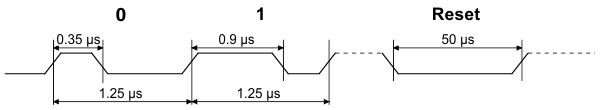
\includegraphics[width=0.8\textwidth]{fig/pololu}
    \caption[LED Specification]{Timing requirements for data transmission to the SK6812 LEDs}
    \label{fig:LEDspec}
\end{figure}

The LED strips WS2812B and SK6812 are controlled with a single data wire, therefore they require precise timing of the data signal for the bit banging. Arduinos are perfectly fine and can generate the required signal on their datapins. Moreover Arduinos are well supported by some open source libraries. Frequently used are Adafruit Neopixel and Fastled. 

Depending on the amount of pixels one LED strip can draw considerable amounts of current. For the chosen RGBW Leds of 4m length with a total of 240 pixel the max current they might draw can be calculated as 240 * 80mA / 1000 = 19,2 Amps. However if the LEDs are programmed appropriately it can be made sure that they do not draw this much power. If it is taken into consideration that Red, Green, Blue, and White are not turned on per pixel at the same time and across the whole strip at once far less current is required. If we plan to use these pixels with just 40mA the estimate current draw is 240 * 40mA /1000 = 9,6 Amps. The pixels are always powered with 5V and the data uses also 5V. Power supplies with 5V and 10 Amps are more widely available and it should also be possible to get these 10 Amps * 5 V = 50 W from a car battery. 

\chapter{Software Prototype}
The software to control the light strips needs the following minimal software components:
Software bit banging for communication with the light strips, pixel mapping for spatially correct presentation, frame selection to merge all current animations by importance, individual animation looping and an event trigger. 

\begin{figure}
    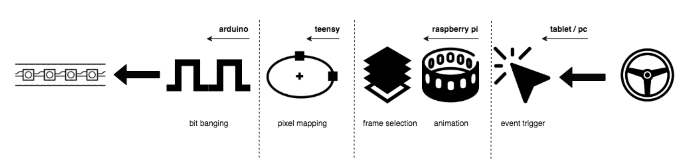
\includegraphics[width=1\textwidth]{fig/softwareflow-}\hfill\
    \caption[Software Flow]{Flow from higher level (right) to lower level software (left)}
    \label{fig:flow}
\end{figure}

In the Figure \fullref{fig:flow} three possible options for separating the lower levels from the higher level software are depicted. This distinction needs to be made because higher processing devices such as PC, tablet and raspberry pi do not have the right hardware interface to communicate with the LED strips; while the microprocessors such as the Arduino and teensy do lack the processing power and graphical interface to realize the application. 
The communication between front and back end is ideally wirelessly and to reduce complexity ideally only one microprocessor and one controller (tablet / pc) should be used.  

\section{Arduino Prototyping}
The first prototype was done with the bare LED strip and an Arduino. To protect the LED strip from damage a few resistors and capacitors need to be wired up\footnote{\url{https://learn.adafruit.com/adafruit-neopixel-uberguide/powering-neopixels}}.  The LEDs proved to be bright enough for peripheral vision during daylight in a car interior. There are a few downsides with prototyping directly on the Arduino: Every change of code needs to be compiled on the PC and uploaded from there to the Arduino; Arduinos have to be programmed in Arduino Style C, floating point calculations can take long and more smooth animations require to be abstracted in mathematical functions. Moreover it is a common practice to save  animations in prepopulated arrays to speed things up. This is not an option for this prototype as animations should be mixed together in real time depending on external inputs. Finally the shape of the Led strips should be taken into account, e.g. animations should not just run from one end of the strip to the other; it should be possible to remap the animations to differently shaped LED strip configurations. 

\section{Processing}

\begin{figure}
    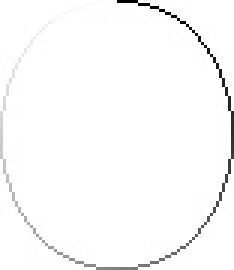
\includegraphics[width=0.3\textwidth]{fig/240id}
    \caption[Pixel Mapping]{Pixel mapping for a LED chain of 240 LEDs to the shape of an ellipse}
    \label{fig:Pixel}
\end{figure}
Instead of rendering the animations on the microprocessor itself they can be rendered on a PC and forwarded to a microprocessor over e.g. the USB port. 
A small application for prototyping with the processing framework was written. This application allows to visualize the animations on screen and send the animations to the Arduino for display on the Led strip. To map the positions of the 2D animation plane to the LED identification number from 0-239 a lookup table was used. The lookup table was created with a modified Bresenham algorithm \cite{MidpointAlgorithm}: we start drawing an ellipse clockwise and increase the ID number with each drawn pixel. In figure \fullref{fig:Pixel} the 78x90 window is depicted and the ellipse that corresponds to the physical configuration of the strip. The resolution of the lookup table depends on the number of Led pixel. Once the lookup table is created it can be stored in some file format e.g. as an image and be reused for each rendered frame. This allows to easily reconfigure the mapping and physical configuration of the light strip. The animations should all be very smooth without stutter and visible edges. Therefore all animations should have a smooth fade to it. When drawing to an animated plane these effects can easily achieved with gradients and colour fades. In processing you can therefore easily draw spherical and rectangular gradients of different sizes colours and transparencies to create animations. Each rendered frame the mapped colour data is send with a simple protocol  facilitating start and end markers over the serial port to the Arduino. Each color is an 8-bit integer. To make space for start and end markers the highest brightness values were omitted. Thus the actively used width per channel are 0-253. Thus, each frame has a payload of 962 bytes. 


\begin{figure}
    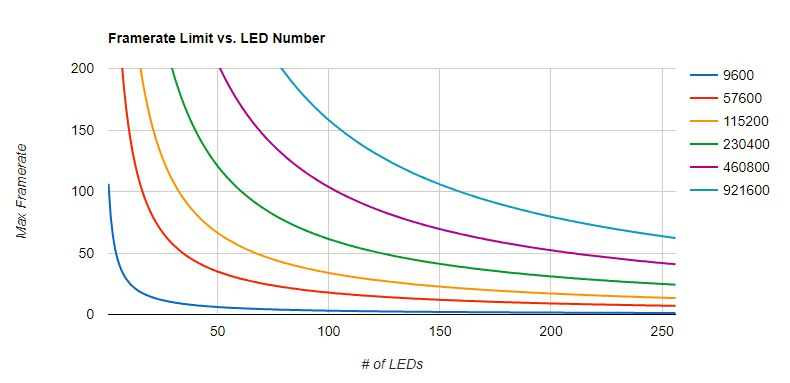
\includegraphics[width=0.8\textwidth]{fig/FPS.JPG}
    \caption[Framerate Limit of RGB LEDs]{Framerate Limit for RGB LED chains with different baudrates. Image adapted from: \url{http://www.partsnotincluded.com/ambilight/calculating-adalight-framerate-limits/}}
    \label{fig:FPS}
\end{figure}

The animations can be drawn and layered with this applications. This allows to test which animation speeds, shapes and colours are distinguishable. Moreover it allowed to easily show these animations to colleagues and refine them so that they can intuitively be understood. One identified shortcoming is the animation speed. Even though the application achieved continuously more than 40 frames per second on the LED strip some fast animations do not feel as smooth as they could be. The provisional conclusion is that, because of the large distance between the pixels, the frame rates of an LED strip should be even higher than the recommended minimal frame rates for displays. Also, the serial port communication with the Arduino in combination with the bit banging with the led strips seems to be a bottleneck; the single threaded Arduino interrupts once a message is received via the serial port and while the pixel colours are dumped to the led strip the serial port is blocked.  This Ambient display has to deliver quick information in a smoothly animated manner; the framerate limitation of the LED chains becomes a severe issue\footnote{\url{http://www.partsnotincluded.com/ambilight/improving-adalight-framerate/}}. 

\section{Bluetooth}
It is not feasible to use a whole Java Processing application on a desktop computer to control the system inside a car; it will be clumsy to control the light signals from a computer and also difficult to integrate it, if so, with the CAN bus of a car. The lowcost Beetle BLE\footnote{\url{https://www.dfrobot.com/wiki/index.php/Bluno_Beetle_SKU:DFR0339}} was used to test if it is feasible to create a wireless system with an Arduino microprocessor. The Beetle Ble has a smaller prototyping board than the Arduino and supports Bluetooth UART communication. This makes it possible to communicate to the Arduino also with a tablet or smartphone device. The processing application was ported to use instead of the usb serial port the bluetooth serial port. The payload for 40 fps is 38,48 Kbyte/s.
Each frame was still rendered by the Java Processing application and then send to the Arduino which just further forwarded the data to the led strip. Unfortunately this approach led to jittered frames as the bluetooth data was not received in order by the Arduino sketch. Multiple approaches did not lead to satisfactory solutions. The implementation of handshaking reduced the frame rate significantly . Using another 16 byte in the payload to signal frame order lead to splitted frame messages; the first half of the message did not always arrive synchronous with the second half. The approach that produced the smoothest transitions was to send messages at a very low frame rate of 10 fps and interpolate all pixel values in between. Even though the transitions were smooth they did not render exactly as intended. E.g. small and fast moving parts do not appear to move quickly across the strip but to light up individual pixels instead. 
\section{Smooth animations}
RGBW Leds are difficult to work with. They are far less common and thus there is less documentation and libraries available. A better choice would have been to use faster LEDs without the white component such as APA102. Even for the slower RGB LEDs without the white component dedicated hardware exists that allows faster and smoother animations. For example the Fadecandy\footnote{\url{https://github.com/scanlime/fadecandy}} and OctoWS2811\footnote{\url{https://github.com/PaulStoffregen/OctoWS2811}} LED Library use a Teensy microprocessor instead of an Arduino; this allows to drive far more LEDs with high frame rate as the communication with multiple LED strips can happen parallely and not serially. Unfortunately these Libraries and hardware configurations usually only support the WS2812 Type of LED strips. DMX via Ethernet is the state of the art protocol for concert light shows. Even with this protocol strips are restricted by the refresh rate of LED strips, speed of data transmission, amount of total pixels and amount of pixels in one chain\footnote{\url{https://support.troikatronix.com/support/solutions/articles/13000042899-controlling-led-strips-via-artnet}}\fnsep\footnote{\url{http://help.madrix.com/tutorials/html/index.html?hidd_dmx_addresses.html}}.  

\section{Raspberry Pi}
To increase the refresh rate up to acceptable smoothness the platform had to be switched. It was chosen to recode the application to run on a raspberry pi. The incentive is to make use of its multithreading capabilities; to do the calculation and mapping of animations as well as the bit banging on the same device. To run the software and hardware on an embedded system delivers the proof that it can be integrated cheaply into a vehicle. This way the only external input to the microprocessor, which is in control of the bit banging, is the event input. Events are only triggered every few seconds instead of milliseconds. Thus the bottleneck of Bluetooth or serial port communication speed is effectively eliminated. 

\section{Pulse Width Modulation}
%more to this maybe
Multithreading is an advantage because multiple processes can run in parallel, however it is an disadvantage too in that it is not straightforward to control the sk6812 LEDs from the raspberry pi platform. The standard GPIO ports are not capable to do the bit banging with the timing that is required by the single wire LED strips. This is the reason why the common LED strip libraries do not support the raspberry pi. However there exists one solution to still get the single wire LED strip to work on a raspberry pi, which is to make use of the pulse width modulation channel of the raspberry pies Broadcom chip. This channel is usually used to create the analogue audio signals for the playback of music. Because the audio playback is stereo, two pulse width modulation channels exist. Thus it is possible to drive two chains of LEDs independently in parallel, which almost doubles the maximal framerates. The only library that is publicly available so far is by Github user Jgarff \cite{Jgarff2018UserspaceLEDs} and fortunately even provides a python wrapper to control the pixel. This is advantageous because then the whole software can be written in one programming language. 


\subsection{CAN Bus}
\label{ssec:CANbus}
The CAN bus is short for Controller Area Network bus developed by Robert Bosch \footnote{\url{https://www.can-cia.org/can-knowledge/can/can-history/}}. It is a standard designed to allow microcontrollers and devices to communicate with each other inside the car without a central computer or huge amount of cables. A lot of car data and sensors are send through this bus system. Interesting for the development of this application are mostly the steering wheel angle, current speed, acceleration, braking force and blinker position. With access to these signals some of the light signals could be automatically triggered and some others could be customized to the current driving conditions. For example the steering wheel angle could be used to tilt the start direction of animations or the blinker could be used to identify when a lane change is about to happen. Unfortunately the Robert Bosch CM department has not the appropriate licence to retrieve all data from the CAN Bus of the Nissan Cube. Robert Bosch works on Clusters and Infotainment for Nissan, thus only the information necessary for these products is available. Unfortunately steering wheel, braking and acceleration are not available. 

The CAN bus is usually not encrypted though, this means that all data is available for a hacker with access to the ports of the car \footnote{\url{https://motherboard.vice.com/en_us/article/ae33jk/we-drove-a-car-while-it-was-being-hacked}}. The difficult part is however to reverse engineer all these messages. Thousands of CAN signals are sent through the network. Thus it is a very time consuming process to find out what the actual bits of signals are depicting.  Almost all software to tap into CAN data is proprietary software from the car industry. The most notable exception is the Panda by Comma.ai ( \fullref{sec:Data}), which is a dongle that plugs into the OBD port of vehicles and streams CAN data to phones or computers. With this dongle and the open source software cabana the CAN data from the Nissan Cube was analysed. The software is capable and helps to reverse engineer CAN Data for hacking vehicles or retrofitting them with self-driving features. The current speed could be extracted from a captured test drive with the Nissan Cube. However open doors, braking and steering wheel angle were not identified. Thus it was decided to not further spend time on this effort before other more significant components got realized. 

\section {Software components}

\begin{figure}
\centering
    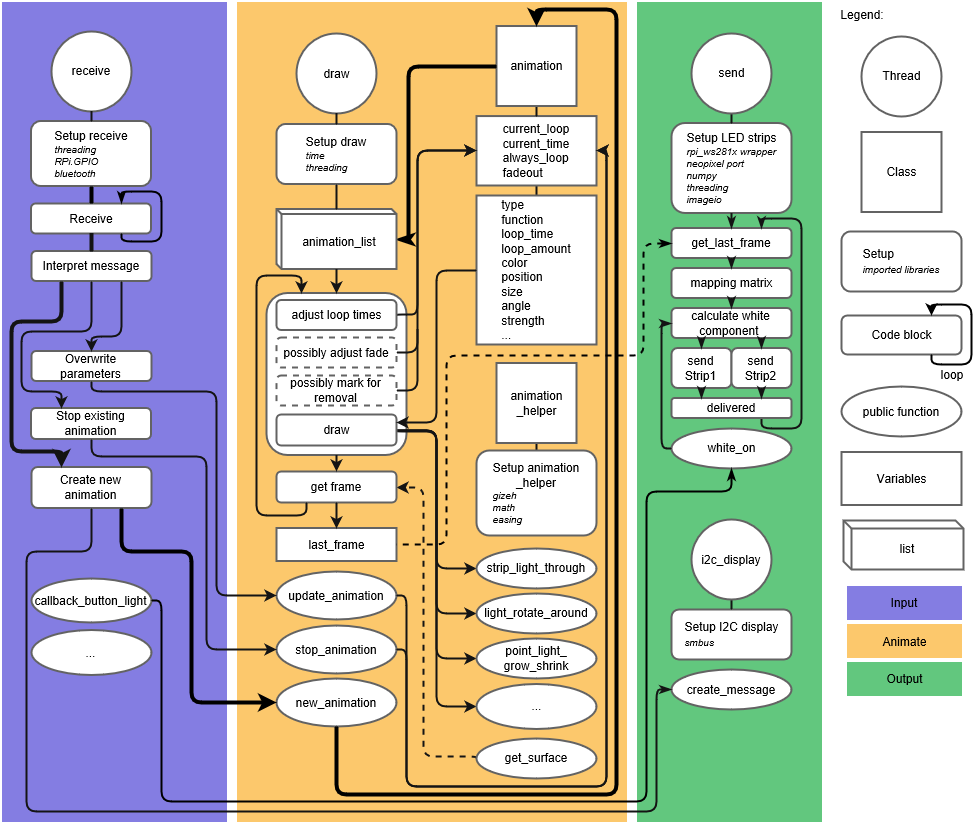
\includegraphics[width=1.12\textwidth]{fig/Flow.png}
    \caption[Software Diagram]{Individual Components of the Application}
    \label{fig:software}
\end{figure}
% This introduction maybe somewhere else
The application is written in python on the raspberry pi. Python was chosen because it the best environment to create all the interface between the individual components. Most importantly the rpi\_ws81x library comes with a python swig wrapper. In production a lower level programming language would be preferable. The application depends on threading because receiving bluetooth messages, sending the data to the light strip, showing messages on the LCD display and rendering the animations should happen independently. If a message comes in the LED strip should not stutter and heavy animations should play frame rate independently. 
In figure \fullref{fig:software} a software overview is shown: In purple the parts that deal with input, in yellow the parts that deal with animation and in green the parts that deal with the output. The three major time consuming loops are ‘receive’ in the receive thread, ‘draw’ in the draw thread and ‘send Strip1’ together with ‘send Strip 2’ in send. The bold line shows the path of an incoming event that gets saved as an animation in the animation\_list. The dotted lines show how the send thread receives the latest animation frame and how the draw class receives an animation frame (surface) from the animation\_helper. 
Receive is the master thread, it set ups the Bluetooth channel and waits for connection of a device. Once it receives a message it interprets the input and calls the appropriate functions in the draw class. Furthermore within 'receive' callback functions for the four arcade buttons are initialized. 
I2C\_display uses the smbus to communicate with a demultiplexer which controls the 8-bit liquid crystal display. The demultiplexer is necessary as otherwise too many GPIO ports from the raspberry pi get blocked. 

The send thread is used for communication with the LED strips. It uses the rpi\_ws18x wrapper for direct memory access for pulse width modulation with the broadcom microprocessor on the Pi. First in the send loop the last animation frame is retrieved from the animation class, then the mapping matrix is applied to filter the animation frame. The mapping matrix is stored in a black \& white image. This way the mapping matrix that was created for the processing application can be reused. Furthermore very specific LED strip shapes could be drawn in graphic applications by hand. For each of the 240 remaining pixels the white component is calculated. The animations are RGB only and the White pixel depends on the reading light button status. Because the animations should be clearly visible even when the reading light is on the white component gets inverse logarithmic dimmed depending on the RGB values. The NumPy library\footnote{\url{http://www.numpy.org/}}is used to speed up matrix operations. The pixel color values are then reorganized as the animation image is RGB but the LED strip is GRBW. The bit patterns are precast in Ram and then transmitted as one entity. 

The draw class takes care of all animations during their lifetime. The public function new\_animation is used to create an instance of animation. All animations are created depending on their type and stored in a list. Each animation has preset values (as  defined in Section \fullref{sec:lightPainting}) such as color, position or loop\_time and values that change during execution such as current\_time. For each drawing iteration each animations loop times in the animation list get updated. The actual drawing is done by the animation\_helper. It uses gizeh\footnote{\url{https://github.com/Zulko/gizeh}}, a vector animation library, math and easing functions for drawing. Multiple options for animations are available via the animation helper. It takes care that consistent looping animations are created but allows to adjust certain variables such as size, color or angle. The animations use transparency so that multiple animations can get overlayed. An possible extension might be to use different blend modes than simple overlays. The light messages are drawn by order of creation. This means that new animations overlay older animations. Once each animation in the list is drawn the full frame is retrieved. Then after a short delay the draw loop starts again. Some animations are stopped manually otherwise they loop forever. When they are stopped and started they get faded in and out. Only after, are they removed from the animation list. 

\section{Wizard Interface}
\label{sec:wizard}
The light signals need to be controlled by a wizard, hence an application or hardware is required to do so. An app was realized with android. It was created for a small tablet so that it can be controlled easily with two hands. Each event can be triggered by its own button. Depending on the type of events these can be triggered once or turned on and off. Furthermore sliders are used to control interval data. Each event button makes use of an descriptive icon, color feedback and text, to help the wizard quickly trigger events. All icons are creative commons and downloaded from \emph{The Noun Project}\footnote{\url{https://thenounproject.com/}}. For transmission of the events a message protocol was created (See Code: \fullref{lst:eventmessage}). These messages are transmitted to the control unit via Bluetooth. 

\begin{lstlisting}[caption={Examples of event messages.},label={lst:eventmessage},language=Python]
<start_moving,loop=1,angle=180>
<brake_now,loop=1,strength=50>
<move_backwards,loop=INF,angle=180>
<move_backwards,loop=OFF>
<highway_enter,loop=3.0>
\end{lstlisting}

The loop can be transmitted as amount of full animation loops \emph{(integer)}, time to play the animation loops \emph{(float)} or as infinite loop duration \emph{(INF, OFF)}. Additional parameters such as angle and strength are send along the event. The wizard can specify them by using the sliders next to event buttons.   
After the first training rounds with the driving wizard and control wizard the buttons in the interface were rearranged according to his preference with the most frequent events close to the left and right border of the screen (See  \fullref{lst:eventmessage}). 

\begin{figure}
    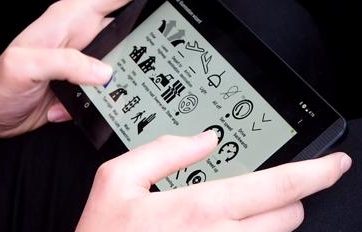
\includegraphics[height=0.31\textwidth]{fig/WizardHands}\hfill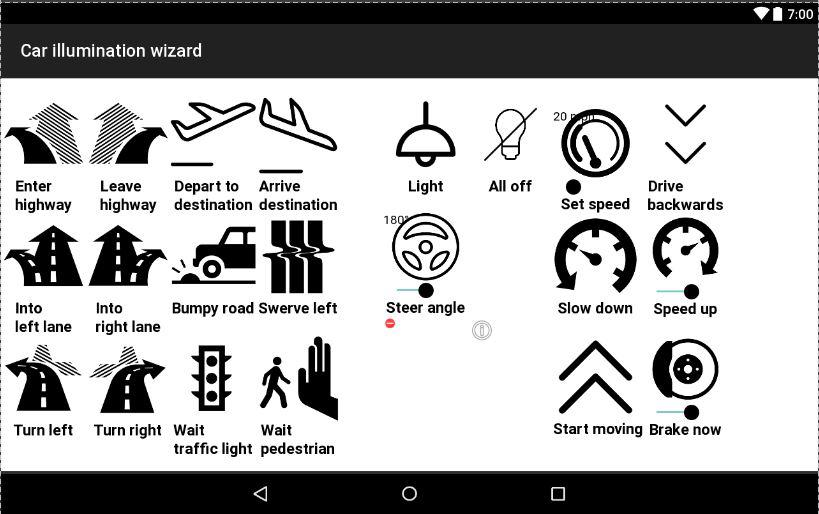
\includegraphics[height=0.31\textwidth]{fig/IlluminationWizard-.JPG}
    \caption[Wizard Tab]{Left: Wizard Tablet. 
   Right: Wizard Interface.}
    \label{fig:wizard}
\end{figure}

\section{Call a Cab App}
\label{sec:capp}
The test subjects should get an idea about what a ride in a potential autonomous cab might look like. For this reason a web app was developed. This app shows the route that will be driven and the participants current location on it. Furthermore the app is used to call the cab to the studies pick up location. This enhances the impression of an autonomous vehicle and disengages the study subjects further from other human contact. The user presses the 'call a cab' button once he is ready to start the test drive and the wizards receive a push notification on their smartphone through the pushbullet service\footnote{\url{https://docs.pushbullet.com/}}. This wizards drive to the pick up location and honk to inform the user of the cabs arrival. 

\begin{figure}
    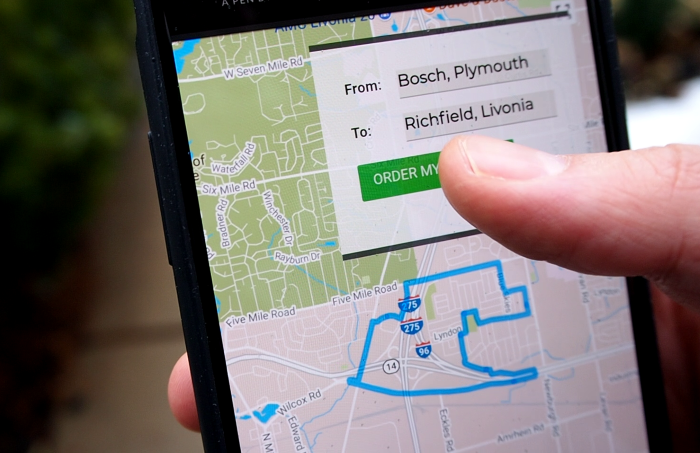
\includegraphics[height=0.31\textwidth]{fig/capp}
    \caption[Call a Cab App]{The web app to call the cab}
    \label{fig:capp}
\end{figure}

\chapter{Physical components}

\begin{figure}
    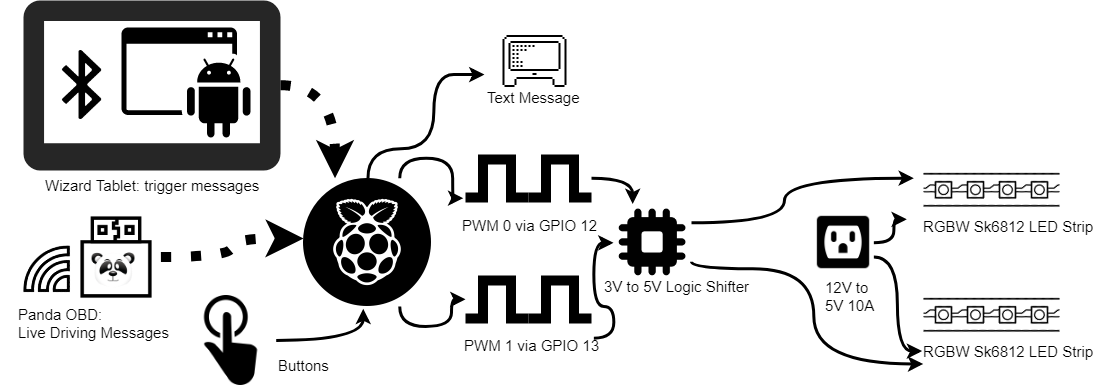
\includegraphics[width=0.8\textwidth]{fig/wizardfinal}
    \caption[Communication Overview]{Communication between individual components}
    \label{fig:communication}
\end{figure}

The  \fullref{fig:communication} shows the hardware connections of the final prototype. The central hub that all devices communicate with is the Raspberry Pi. It uses pulse width modulation to bit bang the colours to the led strip. The led strip is split in half so that each channel controls 120 LED RGBW pixels. The output voltage of the Raspberry Pi GPIO is 3.3 volts. A Logic shifter is used to shift the high voltage bits to 5 volts. The LED strips are powered from the car battery with a step down regulator (12volts regulated to 5volts and 12Amps). The users of the system have access to an emergency stop button, 'Start Ride' button and two buttons for light settings which are connected to the Raspberry Pi with a pull down resistor in place.  The driving events are communicated via an android tab that sends events with Bluetooth to the Raspberry Pi. This allows to easily configure buttons, sliders icons and knobs. The current speed is retrieved via WIFI from the Panda OBD dongle ( \fullref{ssec:CANbus}) A small text display is connected with a port expander to the Raspberry Pi (Sub \fullref{ssec:display}). 

%The capacative touch processor can be used to measure touch input directly on the LED strip. For example touching the light bar could turn on a reading light at that very position. The system should also be connected to the car and acquire data from it such as steering wheel angle, acceleration and brake. These signals are difficult to recreate in real time from a graphical interface. 
\section{Light bar}
\begin{figure}
  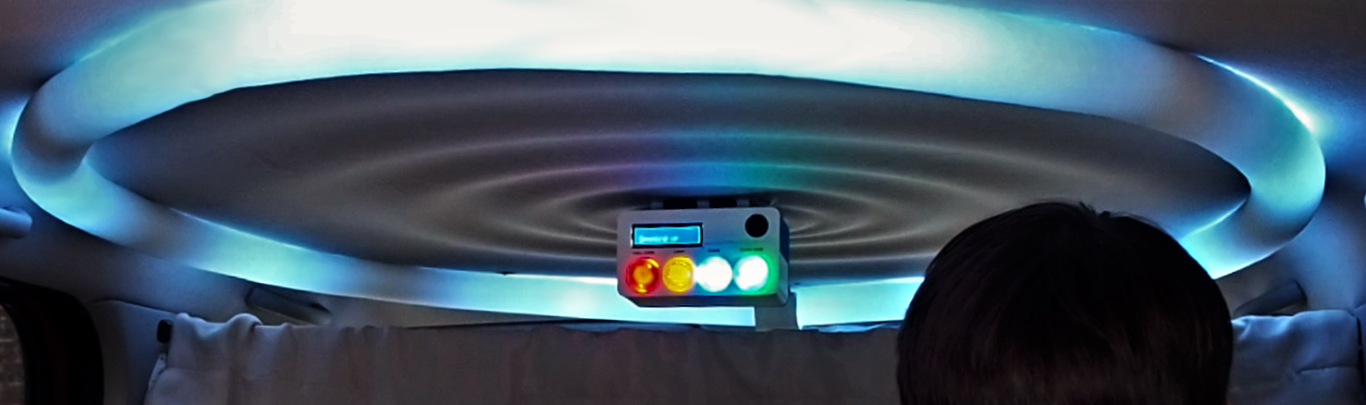
\includegraphics[width=\textwidth]{fig/teaser.png}
  \caption{The ambient display prototype inside the test vehicle (speed up).}
  \label{fig:ambientdisplay}
\end{figure}
The light bar was enclosed by a matte silicon tube. Because it does not diffuse the light enough to obscure individual LED pixels a construction out of semitransparent acrylics was designed ( \fullref{fig:lasercut}). The design files for the laser cutter use 6 sheets of plywood and 6 sheets of diffusing acrylics. The universal snap fit\footnote{\url{https://tltl.stanford.edu/project/universal-snap-fit}} holds the individual sheets together and connects the upper layer wood with the lower layer of acrylics.  Bosch does not have a laser cutter in the Michigan area. Test cuts with a water-jet did not give high-quality edges to justify the cost. A few price estimates from laser cutting companies in the Michigan area were also out of the justifiable price range. 
\begin{figure}
    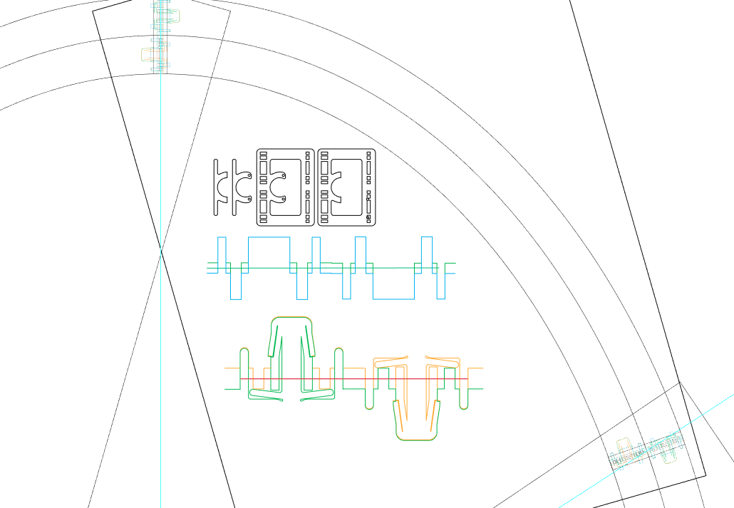
\includegraphics[width=0.8\textwidth]{fig/lasercut.png}
    \caption[Paths for Laser Cutting]{Paths for laser cutting an large ellipse out of diffusing acrylics and plywood sheets (18in x 24in). In the center tube attachments (black), acrylic slots (blue,  enlarged) and interlocking wood mechanism (green and yellow, enlarged) are shown.}
    \label{fig:lasercut}
\end{figure}
Therefore low cost alternative were considered. Insulation foam that is used for pipe insulation diffused the light quite well. This material is also used by cheap LED glow sticks. The two parts of the tube were sewn into the ceiling in the ellipse shape and covered by long sections of the insulation foam. 
In the front the tube, connectors and few electronic parts were covered by a 3d printed housing ( \fullref{fig:boxes}. 

\section{Control Unit}
The raspberry is installed in a housing on the ceiling. It was modeled in a CAD application and then 3D printed. It has cutouts for four arcade buttons, that can be light up, for a liquid crystal display and for a video camera. The layout and placement are inspired by the Waymo self driving vehicles (Fig:\fullref{fig:fig-waymo}). There is a button for starting the ride and for emergency stops (pull over) this might give the passenger a sense of control. Furthermore the Waymo vehicle has a lock doors button and a call for help button. These two were omitted in the favour of a reading light button and an Guide on/off button. 

\begin{figure}
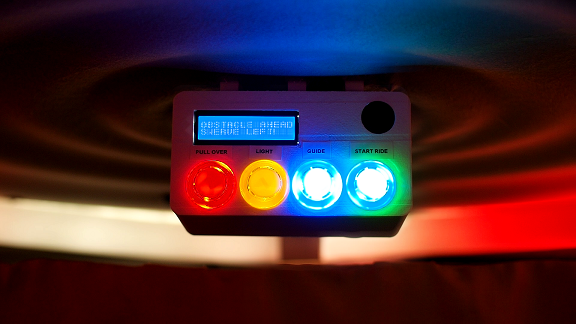
\includegraphics[height=0.38\textwidth]{fig/monitor.png}\hfill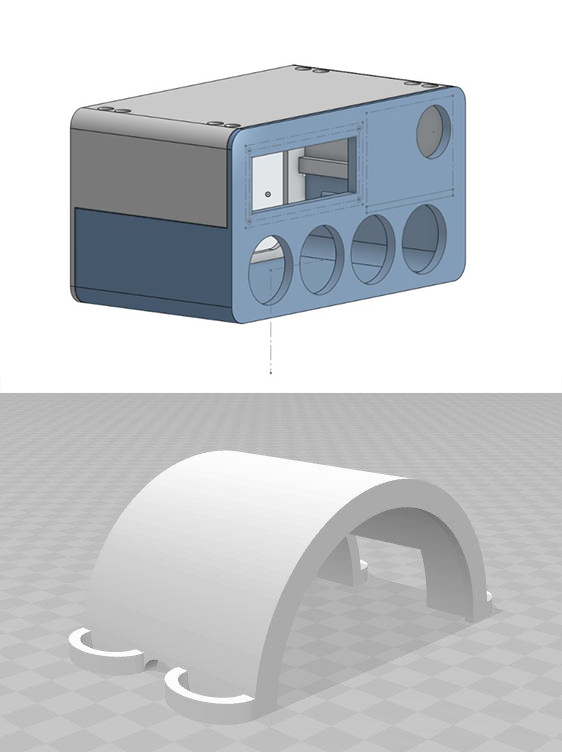
\includegraphics[height=0.38\textwidth]{fig/boxes.jpg}
\caption[Control Unit]{Control unit inside the car prototype with lit-up buttons. CAD files for control unit and foam roll connector.}
    \label{fig:boxes}

\end{figure}

\subsection{Display}
\label{ssec:display}
Because the light display will not be used over a prolonged time by the participants a small display should help the passengers to learn the meaning of the light messages. A LCD display \emph{(HD44780)} was integrated into the control unit. It is connected to the raspberry pi over the I2C protocol. Because it requires a lot of ports for communication 
a port expander was used\footnote{\url{https://www.robotshop.com/letsmakerobots/drive-a-standard-hd44780-lcd-using-a-pcf8574-and-i2c}}. The text messages on the display were triggered by the light messages. The correspondence between light events and display messages is shown in (\fullref{tab:display}).

\begin{table}[ht]
\caption{Correspondence Between Light Events and Display Messages}
\label{tab:display}
\footnotesize
\begin{tabular}{ll}
\toprule
Type        &  Message                      \\
\midrule
turn\_left            & About to turn left           \\
turn\_right           & About to turn right          \\
start\_moving         & Start moving                 \\
move\_backwards       & Driving backwards            \\
lane\_left            & Into: left lane              \\
lane\_right           & Into: right lane             \\
depart\_todestination & Have a good ride!            \\
arrive\_destination   & You arrived!                 \\
highway\_enter        & Entering left                \\
highway\_leave        & Exiting right                \\
wait\_trafficlight    & Waiting for: traffic lights  \\
wait\_pedestrian      & Waiting for: pedestrians     \\
uneven\_road          & Uneven road!                 \\
swerve\_left          & Obstacle ahead: Swerve left! \\
brake\_now            & Braking                      \\
slow\_down            & Slowing down                 \\
speed\_up             & Speeding up                  \\
speed\_keep           & Driving                      \\
default               & Autopilot is active         
\end{tabular}
\end{table}

\subsection{Demonstrator}

\begin{figure}
     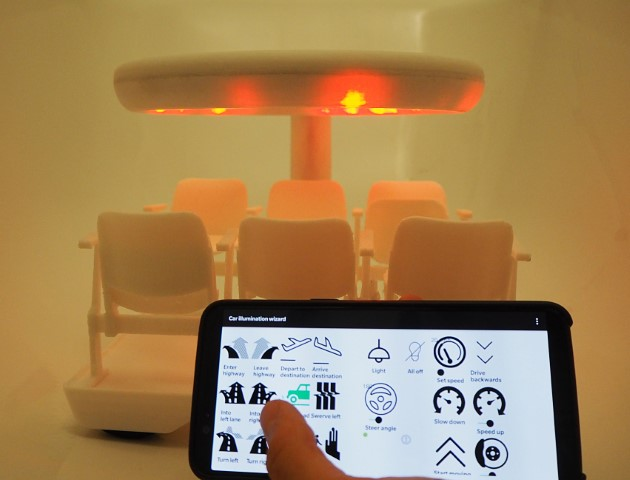
\includegraphics[height=0.36\textwidth]{fig/public.JPG}\hfill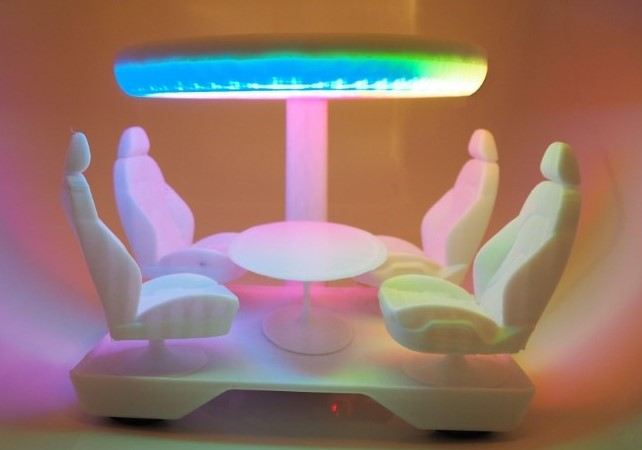
\includegraphics[height=0.36\textwidth]{fig/private.JPG}
    \caption[Desktop Demonstrator]{The miniature demonstrator and control of it (Left:  Public vehicle configuration. Right: Private configuration.)}
    \label{fig:demonstrator}
\end{figure}
\begin{figure}
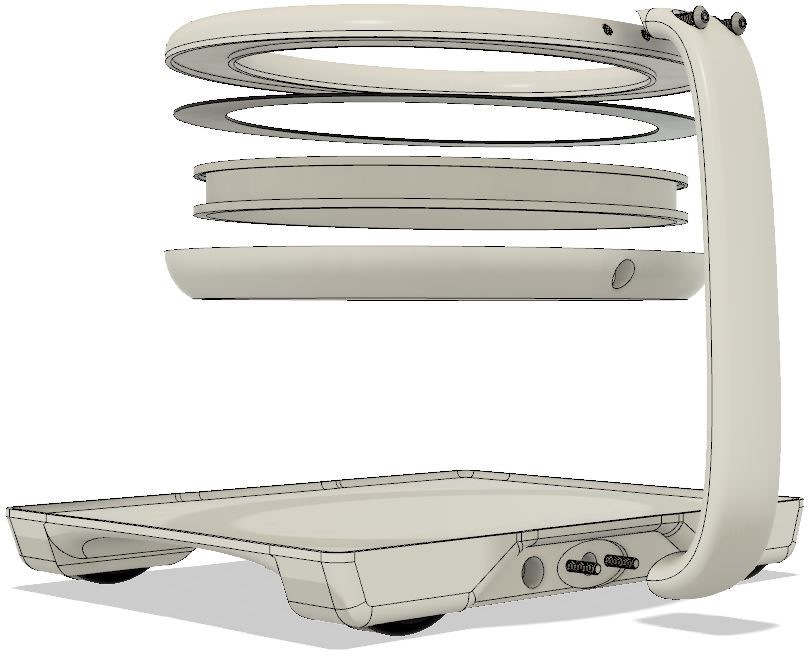
\includegraphics[height=0.38\textwidth]{fig/explosion.JPG}
    \caption[Explosion-view Demonstrator]{Explosion view of the light diffusor}
    \label{fig:demonstratorExplosion}
\end{figure}
During the development of the Light Interface, I spent a lot of time in the test vehicle: for debugging, to fine tune the animations, to add additional functionality and to teach the interaction wizard (See: \fullref{sec:study}) how to use the wizard interface. It is very cumbersome to develop software inside a vehicle because of its inconvenient ergonomics and limited access to infrastructure (power, internet, and heating), this is the first reason why I created the miniature demonstrator ( \fullref{fig:demonstrator}). It can be used next to the work computer. Furthermore, it is useful to have something haptic to show during workshops, exhibitions or to interested partners. Finally, the demonstrator allows car interior designers to test how different interior configurations work together with the light interface. The shape only slightly suggests a vehicle and the open platform provides free positioning of varying seat types, seating arrangements and interior fittings on top of it. The furnishing can get rapidly 3d printed or modeled with traditional methods. The electronics are positioned below it and can be controlled with the Bluetooth Android App ( \fullref{sec:wizard}) or directly plugged into a computer. The 3D printed demonstrator was modeled in Autodesk Fusion 360. The cables pass through the neck which is attached with screws. The light ring consists of 4 parts which are welded together with a 3D pen, and allow the light from two light strips to be redirected downwards through a 3D printed diffusing grid infill. 
